
\documentclass[template=tabling,81pt,headonall]{azmoon}
\usepackage{xepersian}
\usepackage{amsfonts}
\usepackage{graphicx}
\usepackage{svg}
\svgpath{ {./images/} }
\graphicspath{ {./images/} }
\settextfont{Yas}
\setdigitfont{A Iranian Sans}
\usepackage{fontawesome5}

\printanswers
    \teacher{محمد صالح علی اکبری}
    \teachertitle{دبیر}
    \city{رحمت آباد}
    \schooltitle{متوسطه دوره اول}
    \school{مقداد}
    \grade{هفتم}
    \branch{}
    \topic{ریاضی}
    \examdate{۱۳/۰۳/۱۴۰۳}
    \answertime{۸۰ دقیقه}
    \begin{document}
	\begin{questions}
		\nointerlineskip%
		\vskip-\baselineskip
		\question[1.5]{%
حاصل عبارت‌های زیر را بدست آورید: 
    \begin{LTR}
        \begin{parts}[2]\part{$12 + 15 =$}
\part{$14 \times 2 = $}
\part{$8 \div 2 = $}
\part{$14 - 8 = $}
\part{$17 - 8 = $}
\part{$22.5 \div 5 = $}
\end{parts}
\end{LTR}
        
    }\question[1]{%
حاصل عبارت‌های زیر را با رعایت اولویت‌های محاسباتی انجام دهید.
    \begin{LTR}
        \begin{parts}[2]\part{$14 \div 2 \times 3 =$}
\part{$5 + 2 \times 3 =$}
\part{$12 \times 2 \div 3 = $}
\part{$12 \div 3 - 2 = $}
\end{parts}
\end{LTR}
        
    }\question[0.5]{%
حاصل تقسیم‌های زیر را به صورت اعشاری بنویسید.
    \begin{LTR}
        \begin{parts}[1]\part{$72 \div 30 = $}
\part{$15 \div 10 =$}
\end{parts}
\end{LTR}
        
    }\question[1.5]{%
مساحت مثلث زیر را محاسبه کنید. \\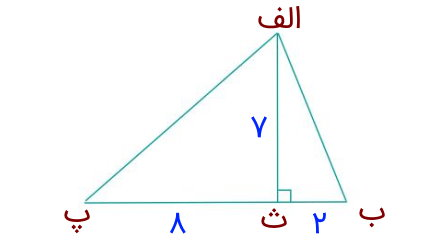
\includegraphics[scale = 0.7]{triangle-area-ex2-1}}\question[2]{%
در مثلث $ABC$ ضلع‌های $BC = 8$ و $AC = 10$ و ارتفاع‌ $AH = 6$ است. طول ارتفاع $BG$ را بدست آورید. \\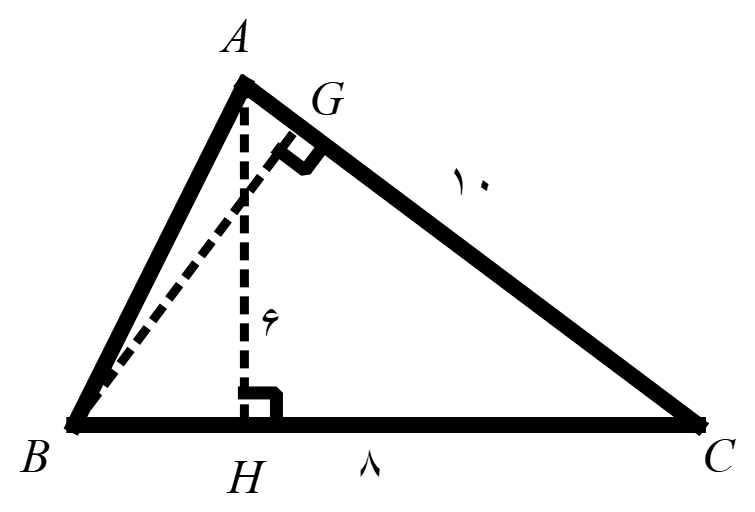
\includegraphics[scale = 0.7]{mosalas_2gh_2h}}\question[6]{%
معادله‌های زیر را حل کنید.
    \begin{parts}[2]\part{$4x + 2 = x + 12$}
\part{$2x + 3 = x + 5$}
‌\\‌\\‌\\\part{$3x + 2 = x + 5$}
\part{$2x + 3 = 4x + 1$}
‌\\‌\\‌\\\part{$3x + 2 = x - 4$}
\part{$5x - 3 = 12x + 2$}
\end{parts}
‌
\\‌
\\‌
\\‌
\\‌
\\
    }\question[2.5]{%
عبارت‌های زیر را محاسبه کنید.
    \begin{LTR}
        \begin{parts}[3]\part{$\sqrt{4}$}
\part{$\sqrt{16}$}
\part{$\sqrt{81}$}
\part{$\sqrt{(-2)^2}$}
\part{$\sqrt{36}$}
\end{parts}
\end{LTR}
        
    }\question[2]{%
ریشه دوم عددهای زیر را محاسبه کنید.
    \begin{parts}[2]\part{$100$}
\part{$25$}
‌\\\part{$9$}
\part{$49$}
\end{parts}
‌
\\
    }\question[3]{%
حاصل عبارت‌های زیر را بدست آورید.
    \begin{LTR}
        \begin{parts}[2]\part{$2^3 - 2^2 = $}
\part{$4^2 \div 2^2 = $}
\part{$2^4 - 3^3 + 1^5 = $}
\end{parts}
\end{LTR}
        ‌
\\
    }\section{یک سؤال ارفاقی}\question[2]{%
حاصل عبارت‌های زیر را محاسبه کنید.
    \begin{LTR}
        \begin{parts}[2]\part{$(\dfrac{5}{2})^2-(\dfrac{2}{5})^2$}
\part{$\sqrt{22 + \sqrt{9}} = $}
\end{parts}
\end{LTR}
        
    }\end{questions}
    \end{document}
    